\documentclass[english,man]{apa6}

\usepackage{amssymb,amsmath}
\usepackage{ifxetex,ifluatex}
\usepackage{fixltx2e} % provides \textsubscript
\ifnum 0\ifxetex 1\fi\ifluatex 1\fi=0 % if pdftex
  \usepackage[T1]{fontenc}
  \usepackage[utf8]{inputenc}
\else % if luatex or xelatex
  \ifxetex
    \usepackage{mathspec}
    \usepackage{xltxtra,xunicode}
  \else
    \usepackage{fontspec}
  \fi
  \defaultfontfeatures{Mapping=tex-text,Scale=MatchLowercase}
  \newcommand{\euro}{€}
\fi
% use upquote if available, for straight quotes in verbatim environments
\IfFileExists{upquote.sty}{\usepackage{upquote}}{}
% use microtype if available
\IfFileExists{microtype.sty}{\usepackage{microtype}}{}

% Table formatting
\usepackage{longtable, booktabs}
\usepackage{lscape}
% \usepackage[counterclockwise]{rotating}   % Landscape page setup for large tables
\usepackage{multirow}		% Table styling
\usepackage{tabularx}		% Control Column width
\usepackage[flushleft]{threeparttable}	% Allows for three part tables with a specified notes section
\usepackage{threeparttablex}            % Lets threeparttable work with longtable

% Create new environments so endfloat can handle them
% \newenvironment{ltable}
%   {\begin{landscape}\begin{center}\begin{threeparttable}}
%   {\end{threeparttable}\end{center}\end{landscape}}

\newenvironment{lltable}
  {\begin{landscape}\begin{center}\begin{ThreePartTable}}
  {\end{ThreePartTable}\end{center}\end{landscape}}

  \usepackage{ifthen} % Only add declarations when endfloat package is loaded
  \ifthenelse{\equal{\string man}{\string man}}{%
   \DeclareDelayedFloatFlavor{ThreePartTable}{table} % Make endfloat play with longtable
   % \DeclareDelayedFloatFlavor{ltable}{table} % Make endfloat play with lscape
   \DeclareDelayedFloatFlavor{lltable}{table} % Make endfloat play with lscape & longtable
  }{}%



% The following enables adjusting longtable caption width to table width
% Solution found at http://golatex.de/longtable-mit-caption-so-breit-wie-die-tabelle-t15767.html
\makeatletter
\newcommand\LastLTentrywidth{1em}
\newlength\longtablewidth
\setlength{\longtablewidth}{1in}
\newcommand\getlongtablewidth{%
 \begingroup
  \ifcsname LT@\roman{LT@tables}\endcsname
  \global\longtablewidth=0pt
  \renewcommand\LT@entry[2]{\global\advance\longtablewidth by ##2\relax\gdef\LastLTentrywidth{##2}}%
  \@nameuse{LT@\roman{LT@tables}}%
  \fi
\endgroup}


  \usepackage{graphicx}
  \makeatletter
  \def\maxwidth{\ifdim\Gin@nat@width>\linewidth\linewidth\else\Gin@nat@width\fi}
  \def\maxheight{\ifdim\Gin@nat@height>\textheight\textheight\else\Gin@nat@height\fi}
  \makeatother
  % Scale images if necessary, so that they will not overflow the page
  % margins by default, and it is still possible to overwrite the defaults
  % using explicit options in \includegraphics[width, height, ...]{}
  \setkeys{Gin}{width=\maxwidth,height=\maxheight,keepaspectratio}
\ifxetex
  \usepackage[setpagesize=false, % page size defined by xetex
              unicode=false, % unicode breaks when used with xetex
              xetex]{hyperref}
\else
  \usepackage[unicode=true]{hyperref}
\fi
\hypersetup{breaklinks=true,
            pdfauthor={},
            pdftitle={Equivalence Testing for Psychological Science},
            colorlinks=true,
            citecolor=blue,
            urlcolor=blue,
            linkcolor=black,
            pdfborder={0 0 0}}
\urlstyle{same}  % don't use monospace font for urls

\setlength{\parindent}{0pt}
%\setlength{\parskip}{0pt plus 0pt minus 0pt}

\setlength{\emergencystretch}{3em}  % prevent overfull lines

\ifxetex
  \usepackage{polyglossia}
  \setmainlanguage{}
\else
  \usepackage[english]{babel}
\fi

% Manuscript styling
\captionsetup{font=singlespacing,justification=justified}
\usepackage{csquotes}
\usepackage{upgreek}

 % Line numbering
  \usepackage{lineno}
  \linenumbers


\usepackage{tikz} % Variable definition to generate author note

% fix for \tightlist problem in pandoc 1.14
\providecommand{\tightlist}{%
  \setlength{\itemsep}{0pt}\setlength{\parskip}{0pt}}

% Essential manuscript parts
  \title{Equivalence Testing for Psychological Science}

  \shorttitle{Equivalence Testing}


  \author{Daniel Lakens\textsuperscript{1}, Anne M. Scheel\textsuperscript{1}, \& Peder Isager\textsuperscript{1}}

  \def\affdep{{"", "", ""}}%
  \def\affcity{{"", "", ""}}%

  \affiliation{
    \vspace{0.5cm}
          \textsuperscript{1} Eindhoven University of Technology  }

  \authornote{
    \newcounter{author}
    We would like to thank Courtney Soderbergh for creating the first
    version of the TOST function to test two independent proportions.

                      Correspondence concerning this article should be addressed to Daniel Lakens, Den Dolech 1, IPO 1.33, 5600 MB, Eindhoven, The Netherlands. E-mail: \href{mailto:D.Lakens@tue.nl}{\nolinkurl{D.Lakens@tue.nl}}
                                    }


  \abstract{Psychologists need to be able to test for the absence of an effect.
Using the Two-One-Sided Tests (TOST) procedure, researchers can easily
test whether the observed effects are too small to be meaningful. By
specifying a smallest effect size of interest (SESOI) researchers test
whether observed effects are surprisingly closer to zero, assuming there
was an effect the consider meaningful. We explain a range of approaches
to determine the SESOI in psychological science, and provide detailed
examples of how equivalence tests should be performed and reported.}
  \keywords{Equivalence Testing, NHST, power, TOST \\

    \indent Word count: X
  }





\usepackage{amsthm}
\newtheorem{theorem}{Theorem}
\newtheorem{lemma}{Lemma}
\theoremstyle{definition}
\newtheorem{definition}{Definition}
\newtheorem{corollary}{Corollary}
\newtheorem{proposition}{Proposition}
\theoremstyle{definition}
\newtheorem{example}{Example}
\theoremstyle{definition}
\newtheorem{exercise}{Exercise}
\theoremstyle{remark}
\newtheorem*{remark}{Remark}
\newtheorem*{solution}{Solution}
\begin{document}

\maketitle

\setcounter{secnumdepth}{0}



Psychologists should be able to falsify predictions. A common prediction
in psychological research is that an effect exists in the population
that differs from zero. For example, we might predict that priming
American Asian women with their Asian identity will increase their
performance on a math test compared to women who are primed with their
female identity. To be able to falsify this hypothesis, and design a
study that allows for strong inferences ({\textbf{???}}), it is
important to specify which test result would \emph{disprove} the
hypothesis.

An equivalence test can be used to test whether the observed effect is
surprisingly small, assuming a meaningful effect exists in the
population. The test is a simple variation of the widely used null
hypothesis significance tests (NHST). To understand the idea behind
equivalence tests, it is useful to realize the null hypothesis we test
against can be any numerical value. When we compare two groups, we often
test whether the difference between these groups is zero, but we may
sometimes want to test against other values than zero. Imagine a
researcher who is interested in voluntary participation in a national
program to train young infants' motor skills. The researcher wants to
test whether more boys than girls are brought into the program by their
parents. One could test whether the difference between boys and girls is
zero. However, this would ignore the fact that the human sex ratio of
newborn boys to girls is not exactly 1:1, and we should not expect 50\%
of participants to be boys. On average, 103 boys are born for every 100
girls (CIA, 2017), so approximately 50.74\% of applicants should be
boys, and 49.26\% should be girls (with 0.5074/0.4926≈1.03). If boys and
girls were exactly equally likely to be brought into the program by
their parents, we would not expect a difference of zero, but 1.5\% more
boys. This can be used as a null hypothesis: Rather than testing against
a difference in proportions of 0, the researcher tests against 0.015.

Even though 0.015 might be a more sensible value for a null hypothesis,
our researcher knows that the true sex ratio in their population will
differ slightly from that in the entire world. Rather than testing a
point null hypothesis (setting \(H_0\) to one specific value), the
researcher decides to define a range of values around the difference in
proportions of 0.015 that can be considered trivially small, even when
the true ratio in the population is not exactly 0, or even 0.015. The
researcher can for example test if the difference is smaller than
-0.005, or larger than 0.035. This test against two bounds, with \(H_0\)
as a range rather than one value, is known as a \emph{minimal effects
test} (Murphy, Myors, \& Wolach, 2014).(Murphy et al. 2014)

However, even if the researcher would consider any difference in
percentages smaller than \(-0.5 \%\) or larger than \(3.5 \%\) a
rejection of the null hypothesis, not every difference is large enough
to matter in practice. As long as gender differences in the
participation rate are not too extreme, there is no need to spend money
to address the gender imbalance in the voluntary participation rate, and
all money can be spent on the core training program. To test whether the
gender difference in participants is not large enough to matter, the
researcher can perform an \emph{equivalence test}. Equivalence tests
examine whether the presence of gender differences that are large enough
to matter can be rejected. After an extensive discussion with experts,
the researcher decides that as long as the difference in proportions is
not larger than 6\% the researcher can act as if the gender difference
is too small to intervene. Given an expected true difference in the
population of 0.015, the researcher will tests if the observed
difference in the data is smaller than 0.075, and larger than -0.055. If
differences more extreme than both these boundary values can be rejected
in two one-sided tests, the researcher will conclude statistical
equivalence, and no money will be spent on addressing a gender
difference in participation.

One can conclude statistical equivalence whenever a 90\% confidence
interval around the observed estimate does not contain the smallest
effect size of interest (SESOI). Figure 1 illustrates the possible
conclusions we can draw from null hypothesis, minimal effect, and
equivalence tests.

Even though equivalence tests are just a small variation of traditional
frequentist null-hypothesis significance tests (and test against the
SESOI, instead of a value of 0), their use was limited until the
availability of user-friendly software to perform the calculations
(Lakens, 2017). In this article, we provide several examples of
equivalence tests which illustrate the procedure. Furthermore, we
discuss different approaches to determining the SESOI for psychological
research, and provide detailed reproducible examples of how to perform
power analyses when designing equivalence tests, and statistical
re-analyses of published psychology experiments.

\section{Justifying the Smallest Effect Size of
Interest}\label{justifying-the-smallest-effect-size-of-interest}

Equivalence tests are performed against a value that is considered the
smallest effect size of interest (SESOI). The SESOI can sometimes be
based on just noticeable differences, which can be objectively
determined. Most often, however, it is a subjective decision that varies
across individuals and time. The SESOI is ideally based on a
cost-benefit analysis. Since both costs and benefits are necessarily
subjective, the SESOI will depend on the researcher who designs the
study. The goal of setting a SESOI is to clearly justify why designing a
study that has a high probability of rejecting effects larger than a
specified value contributes to our knowledge base. A SESOI should be
chosen such that inferences based on it answer a meaningful question.

\subsection{Objective Justifications of a
SESOI}\label{objective-justifications-of-a-sesoi}

An objectively determined SESOI should be based on quantifiable
theoretical predictions, such as computational models. Sometimes, the
only theoretical prediction is that an effect should be noticeable. In
such circumstances, the SESOI can be set based on just noticeable
differences. For example, Burriss and colleagues ({\textbf{???}})
examined whether women displayed an increase in redness in the face
during the fertile phase of their ovulatory cycle. The hypothesis was
that a slightly redder skin signals greater attractiveness and physical
health, and sending this signal to men yields an evolutionary advantage.
This hypothesis requires that the increase in redness can be detected
with the naked eye by men. They collected data from 22 women and showed
that there was indeed an increase in redness of the facial skin of woman
during their fertile period. However, this increase was not large enough
to be noticeable with the naked eye by men, thus falsifying their
hypothesis. Because the just noticeable difference in redness of the
skin can be measured, it is possible to objectively establish the SESOI.

Another example of an objectively determined SESOI can be found in
({\textbf{???}}) where the minimal clinically important difference on
the Beck Depression Inventory - II was determined by asking 1039
patients when they subjectively felt less depressed (i.e., when they
personally noticed an improvement) and relating this to the
corresponding difference score on the depression inventory.

\subsection{Subjective justifications of a
SESOI}\label{subjective-justifications-of-a-sesoi}

We distinguish between three categories of subjective justifications for
SESOI. First, researchers can use benchmarks. For example, one might set
the SESOI to a standardized effect size of d = 0.5, which would allow
one to reject effect as large or larger than a \enquote{medium} effect
size (Cohen, 1988). Similarly, effect sizes smaller than a Cohen's d of
0.1 are sometimes considered trivially small (Maxwell, Lau, \& Howard,
2015). Relying on a benchmark is the weakest possible justification of a
SESOI, and should be avoided.

Second, researchers can determine the SESOI based on previous work in
the literature. Ideally, researchers would specify their SESOI in
studies they report, but this is not yet common practice. It is thus up
to researchers who build on earlier work to decide which effect size is
too small to be meaningful, given an earlier study. Simonsohn (2015)
recently proposed to set the SESOI to the effect size that an earlier
study on the same effect would have 33\% power to detect based on the
sample size. This is called the \enquote{small telescopes} approach. For
example, consider a study where 100 participants answered a question,
which was analyzed with an one-sample t-test. For a two-sided test with
an alpha of 0.05 this test had 33\% power to detect a d = 0.15.

Another justifiable choice for the SESOI we would like to propose here
is to use the smallest observed effect size that could have been
statistically significant in the original study. In other words, we
decide that effects that could not have yielded a \emph{p} \textless{}
0.05 in the original study (if this is your preferred alpha threshold)
will not be considered meaningful in the replication either, even if
effects of this size are statistically significant in the replication
study. Based only on the alpha level and the sample size, we can
calculate the critical test value (e.g., \emph{t}, \emph{F}, \emph{Z}).
This critical test value can also be transformed to a standardized
effect size (e.g.,
\(d = t \sqrt { \frac { 1} { n _ { 1} } + \frac { 1} { n _ { 2} } }\)),
which can thus be interpreted as a \emph{critical effect size}. All
observed effect sizes smaller than the critical effect size would not be
statistically significant in an original study, given the alpha and
sample size of that study. By setting the SESOI to the critical effect
size, an equivalence test can reject all observed effect sizes that
could have been detected in an earlier study.

Third, researchers can set the SESOI based on the resources they have
available. The amount of data you can collect limits the inferences you
can make. Given a an alpha level and a sample size, researchers can
calculate the smallest effect size that one has sufficient power to
detect. This approach is suggested here to provide researchers with a
way to think about setting the SESOI for a study in a line of research
where no quantifiable predictions are made, and where no previous
studies have been performed. Observing statistical equivalence for a
SESOI based on this approach allows one to reject effects that can be
reliably detected with the given sample size. For example, a researcher
who plans to perform a two-sided one-sample \emph{t}-test using an alpha
of 5\%, based on data from 100 observations, has 90\% power to detect an
effect of d = 0.364. Using equivalence bounds of d = -0.364 and d =
0.364 in an equivalence test allows one to reject effects the study had
high statistical power to detect. In this case, concluding equivalence
would suggest one can reject effects that can reasonably be detected
with N = 100. Whether or not this is interesting depends in part on how
typical the chosen sample size is for a research area. One should not
expect an equivalence test based on 15 observations testing against a
SESOI of d = -1 and d = 1 to substantially increase our knowledge, given
that most effects in psychology are substantially smaller than these
bounds. But by transparently reporting the effects one can detect and
reject, based on the study design, researchers can communicate the
information their study contributes. When there are no previous studies
to build on, and no theoretical predictions, specifying a SESOI based on
the alpha level and a sample size can provide a starting point for a
discussion on what a reasonable SESOI is. Nevertheless, the value of
setting a SESOI based on this procedure is limited, and the equivalence
test does not reject values that are theoretically interesting.

\subsection{Example 1: Statistically Equivalent and Not Statistically
Different}\label{example-1-statistically-equivalent-and-not-statistically-different}

Banerjee, Chatterjee, \& Sinha (2012) reported that participants who had
been asked to describe an unethical deed from their past judged the room
to be darker than participants who had been asked to describe an ethical
deed (\(M_{unethical}= 4.71\), \({SD}_{unethical}= 0.85\),
\(M_{ethical}=5.30\), \({SD}_{ethical}=0.97\), \(t(38)= 2.03\),
\(p= 0.05\), \(d= 0.65\)). A close replication by Brandt, IJzerman, \&
Blanken (2014) found no significant effect (\(t(98)=0.56\), \(p=0.57\),
\(d=0.11\)). The smallest effect size that could have been statistically
significant in the original study is
\(d_{crit}= 2.02 \sqrt { \frac { 1} {20} + \frac { 1} {20} }=0.64\).
Using this as our SESOI for a TOST with Welch's \emph{t}-test for
independent samples --- resulting in equivalence bounds of
\({\Delta}_L=-0.64\) and \({\Delta}_U=0.64\) --- we indeed find that the
effect reported by the replication study is statistically equivalent,
\(t(97.78)=-2.64\), \(p=0.00\).

\begin{figure}[htbp]
\centering
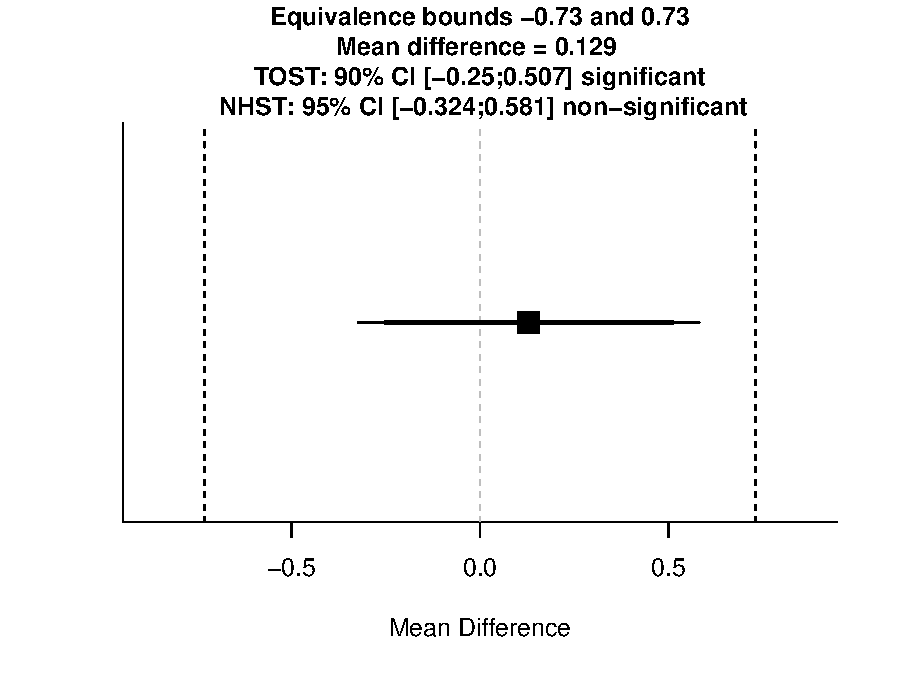
\includegraphics{manuscript_files/figure-latex/unnamed-chunk-6-1.pdf}
\caption{}
\end{figure}

\begin{verbatim}
## Using alpha = 0.05 Welch's t-test was non-significant, t(97.78283) = 0.5649507, p = 0.5734012
## Using alpha = 0.05 the equivalence test based on Welch's t-test  was significant, t(97.78283) = -2.638058, p = 0.004851125TOST results:
##   t-value 1    p-value 1 t-value 2   p-value 2       df
## 1   3.76796 0.0001407233 -2.638058 0.004851125 97.78283
## 
## Equivalence bounds (Cohen's d):
##   low bound d high bound d
## 1  -0.6401696    0.6401696
## 
## Equivalence bounds (raw scores):
##   low bound raw high bound raw
## 1    -0.7302364      0.7302364
## 
## TOST confidence interval:
##   Lower Limit 90% CI raw Upper Limit 90% CI raw
## 1              -0.249788               0.507388
\end{verbatim}

\subsection{Example 2: Statistically Equivalent and Statistically
Different}\label{example-2-statistically-equivalent-and-statistically-different}

\begin{figure}[htbp]
\centering
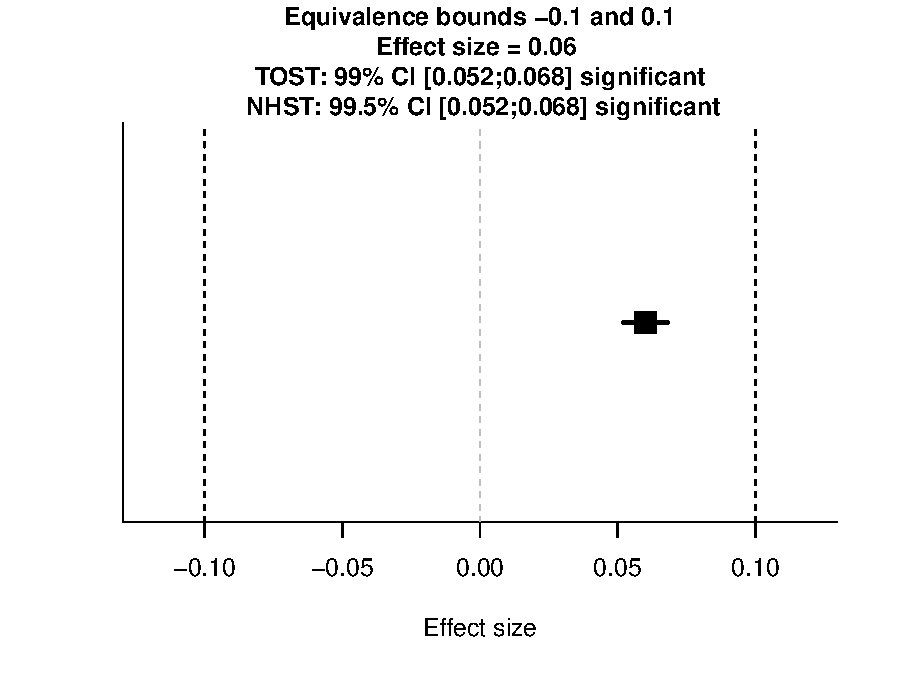
\includegraphics{manuscript_files/figure-latex/unnamed-chunk-7-1.pdf}
\caption{}
\end{figure}

\begin{verbatim}
## Using alpha = 0.005 the meta-analysis was significant, Z = 20, p = 5.507248e-89
## Using alpha = 0.005 the equivalence test was significant, Z = -13.33333, p = 7.406413e-41TOST results:
##   Z-value 1 p-value 1 Z-value 2    p-value 2
## 1  53.33333         0 -13.33333 7.406413e-41
## 
## Equivalence bounds (Cohen's d):
##   low bound d high bound d
## 1        -0.1          0.1
## 
## TOST confidence interval:
##   Lower Limit 99% CI Upper Limit 99% CI
## 1         0.05227251         0.06772749
\end{verbatim}

\begin{figure}[htbp]
\centering
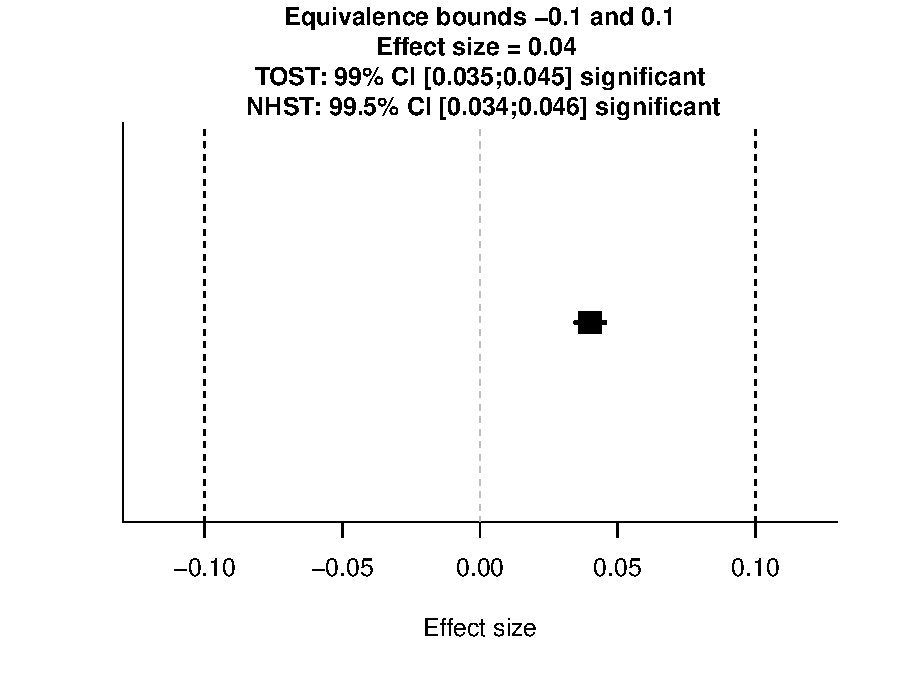
\includegraphics{manuscript_files/figure-latex/unnamed-chunk-7-2.pdf}
\caption{}
\end{figure}

\begin{verbatim}
## Using alpha = 0.005 the meta-analysis was significant, Z = 20, p = 5.507248e-89
## Using alpha = 0.005 the equivalence test was significant, Z = -30, p = 4.906714e-198TOST results:
##   Z-value 1 p-value 1 Z-value 2     p-value 2
## 1        70         0       -30 4.906714e-198
## 
## Equivalence bounds (Cohen's d):
##   low bound d high bound d
## 1        -0.1          0.1
## 
## TOST confidence interval:
##   Lower Limit 99% CI Upper Limit 99% CI
## 1         0.03484834         0.04515166
\end{verbatim}

\begin{figure}[htbp]
\centering
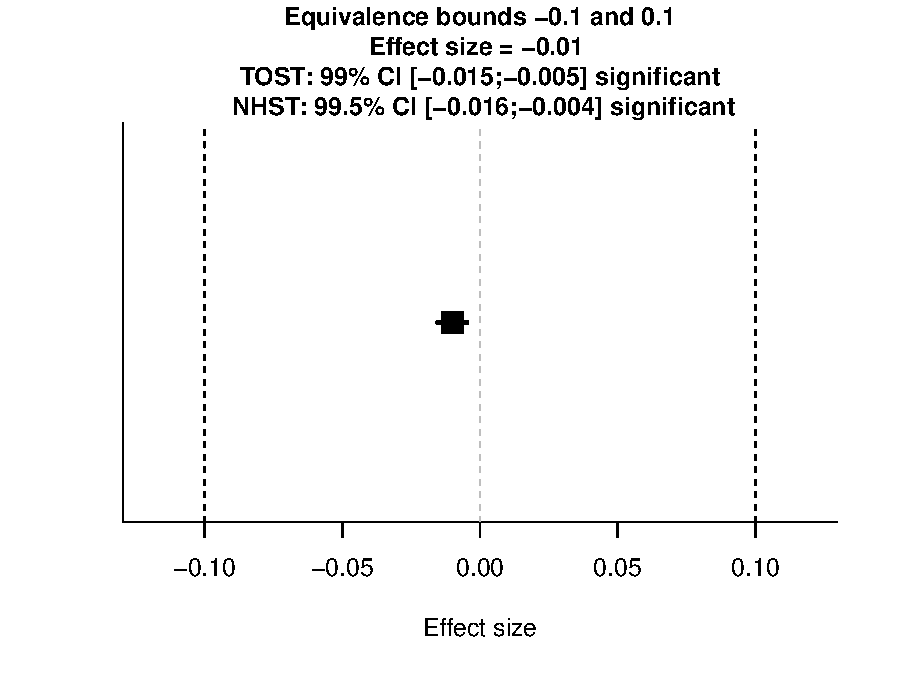
\includegraphics{manuscript_files/figure-latex/unnamed-chunk-7-3.pdf}
\caption{}
\end{figure}

\begin{verbatim}
## Using alpha = 0.005 the meta-analysis was significant, Z = -5, p = 5.733031e-07
## Using alpha = 0.005 the equivalence test was significant, Z = 45, p = 0TOST results:
##   Z-value 1 p-value 1 Z-value 2 p-value 2
## 1        45         0       -55         0
## 
## Equivalence bounds (Cohen's d):
##   low bound d high bound d
## 1        -0.1          0.1
## 
## TOST confidence interval:
##   Lower Limit 99% CI Upper Limit 99% CI
## 1        -0.01515166       -0.004848341
\end{verbatim}

\begin{verbatim}
## Using alpha = 0.005 the meta-analysis was significant, Z = -5, p = 5.733031e-07
## Using alpha = 0.005 the equivalence test was significant, Z = 45, p = 0TOST results:
##   Z-value 1 p-value 1 Z-value 2 p-value 2
## 1        45         0       -55         0
## 
## Equivalence bounds (Cohen's d):
##   low bound d high bound d
## 1        -0.1          0.1
## 
## TOST confidence interval:
##   Lower Limit 99% CI Upper Limit 99% CI
## 1        -0.01515166       -0.004848341
\end{verbatim}

\begin{verbatim}
## Using alpha = 0.005 the meta-analysis was significant, Z = -5, p = 5.733031e-07
## Using alpha = 0.005 the equivalence test was significant, Z = 45, p = 0TOST results:
##   Z-value 1 p-value 1 Z-value 2 p-value 2
## 1        45         0       -55         0
## 
## Equivalence bounds (Cohen's d):
##   low bound d high bound d
## 1        -0.1          0.1
## 
## TOST confidence interval:
##   Lower Limit 99% CI Upper Limit 99% CI
## 1        -0.01515166       -0.004848341
\end{verbatim}

\begin{figure}[htbp]
\centering
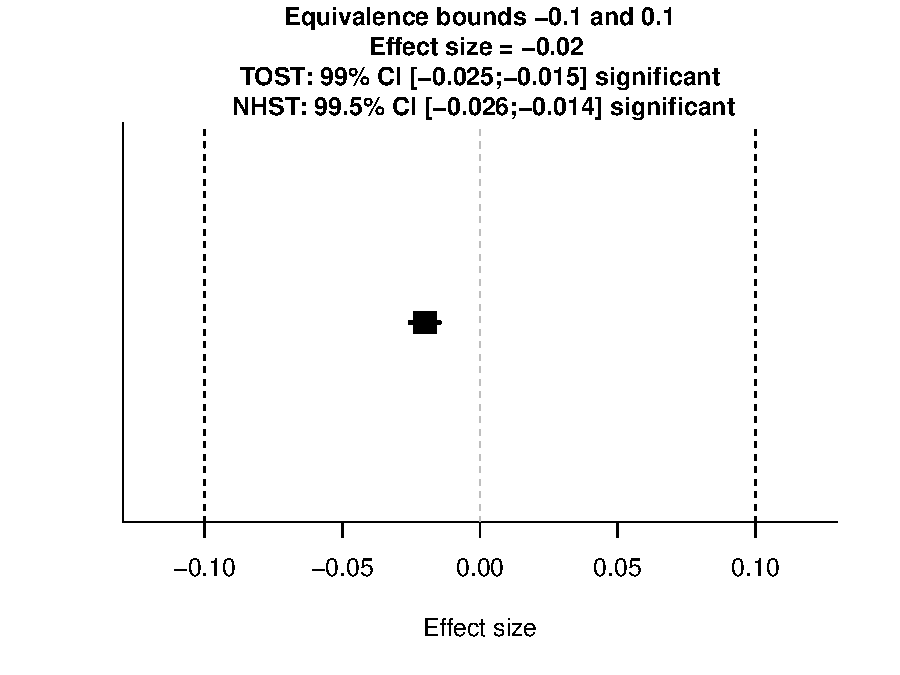
\includegraphics{manuscript_files/figure-latex/unnamed-chunk-7-4.pdf}
\caption{}
\end{figure}

\begin{verbatim}
## Using alpha = 0.005 the meta-analysis was significant, Z = -10, p = 1.523971e-23
## Using alpha = 0.005 the equivalence test was significant, Z = 40, p = 0TOST results:
##   Z-value 1 p-value 1 Z-value 2 p-value 2
## 1        40         0       -60         0
## 
## Equivalence bounds (Cohen's d):
##   low bound d high bound d
## 1        -0.1          0.1
## 
## TOST confidence interval:
##   Lower Limit 99% CI Upper Limit 99% CI
## 1        -0.02515166        -0.01484834
\end{verbatim}

\begin{verbatim}
## Using alpha = 0.005 the meta-analysis was significant, Z = -10, p = 1.523971e-23
## Using alpha = 0.005 the equivalence test was significant, Z = 40, p = 0TOST results:
##   Z-value 1 p-value 1 Z-value 2 p-value 2
## 1        40         0       -60         0
## 
## Equivalence bounds (Cohen's d):
##   low bound d high bound d
## 1        -0.1          0.1
## 
## TOST confidence interval:
##   Lower Limit 99% CI Upper Limit 99% CI
## 1        -0.02515166        -0.01484834
\end{verbatim}

\begin{figure}[htbp]
\centering
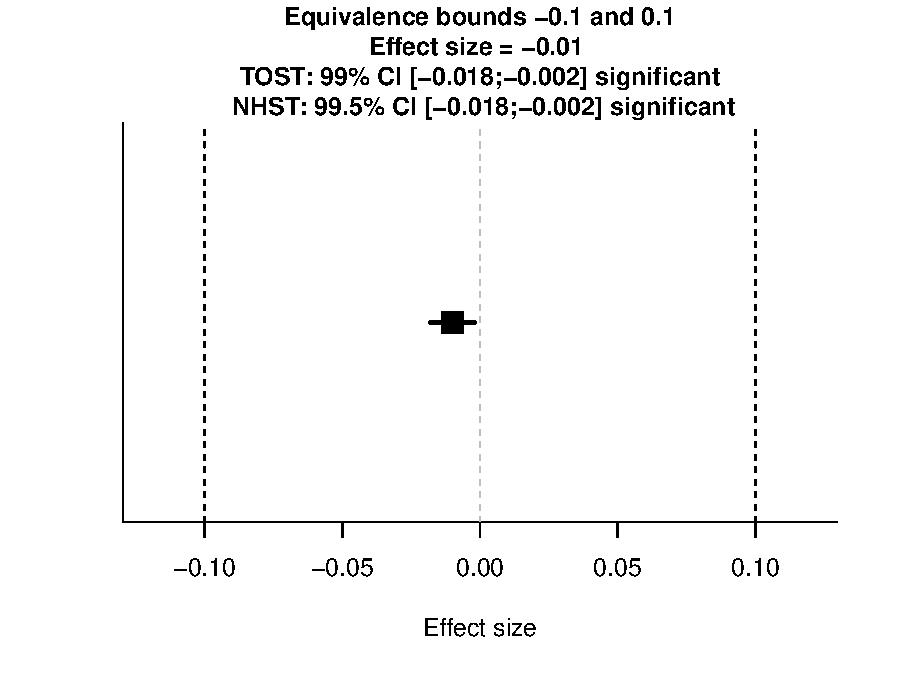
\includegraphics{manuscript_files/figure-latex/unnamed-chunk-7-5.pdf}
\caption{}
\end{figure}

\begin{verbatim}
## Using alpha = 0.005 the meta-analysis was significant, Z = -3.333333, p = 0.0008581207
## Using alpha = 0.005 the equivalence test was significant, Z = 30, p = 4.906714e-198TOST results:
##   Z-value 1     p-value 1 Z-value 2     p-value 2
## 1        30 4.906714e-198 -36.66667 1.241408e-294
## 
## Equivalence bounds (Cohen's d):
##   low bound d high bound d
## 1        -0.1          0.1
## 
## TOST confidence interval:
##   Lower Limit 99% CI Upper Limit 99% CI
## 1        -0.01772749       -0.002272512
\end{verbatim}

\begin{figure}[htbp]
\centering
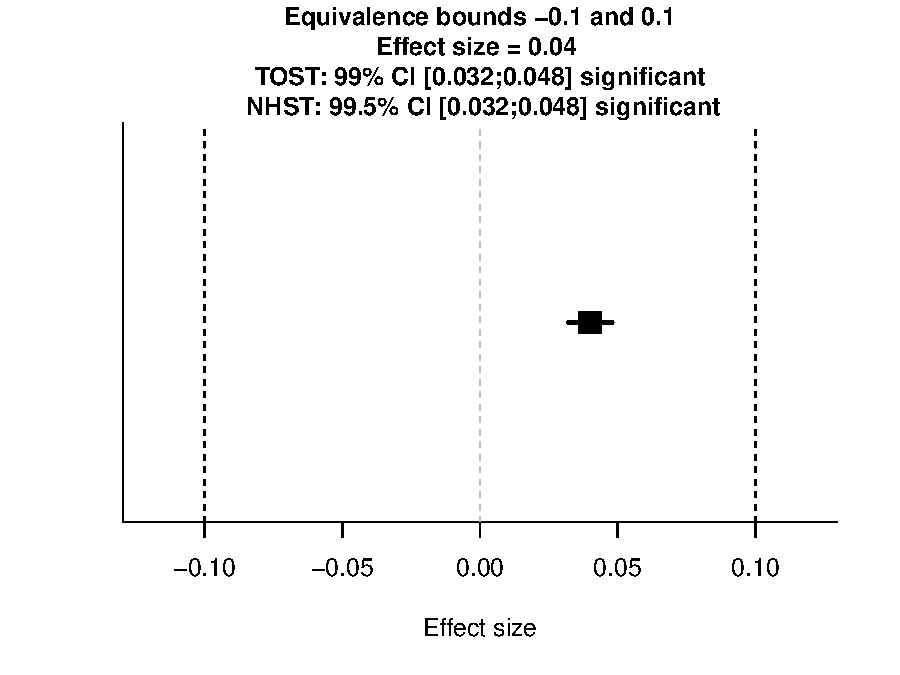
\includegraphics{manuscript_files/figure-latex/unnamed-chunk-7-6.pdf}
\caption{}
\end{figure}

\begin{verbatim}
## Using alpha = 0.005 the meta-analysis was significant, Z = 13.33333, p = 1.481283e-40
## Using alpha = 0.005 the equivalence test was significant, Z = -20, p = 2.753624e-89TOST results:
##   Z-value 1 p-value 1 Z-value 2    p-value 2
## 1  46.66667         0       -20 2.753624e-89
## 
## Equivalence bounds (Cohen's d):
##   low bound d high bound d
## 1        -0.1          0.1
## 
## TOST confidence interval:
##   Lower Limit 99% CI Upper Limit 99% CI
## 1         0.03227251         0.04772749
\end{verbatim}

\begin{figure}[htbp]
\centering
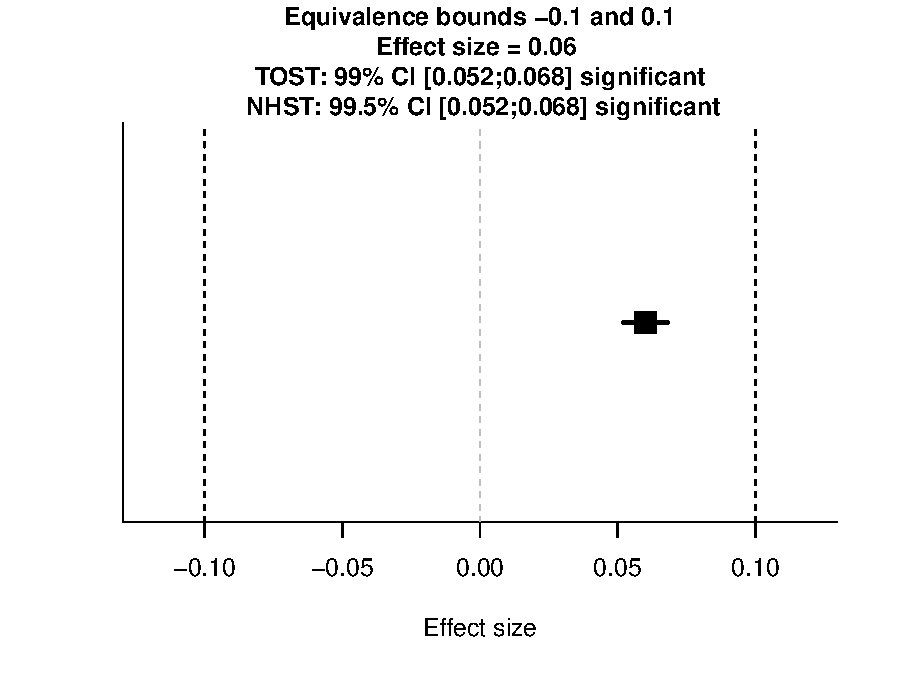
\includegraphics{manuscript_files/figure-latex/unnamed-chunk-7-7.pdf}
\caption{}
\end{figure}

\begin{verbatim}
## Using alpha = 0.005 the meta-analysis was significant, Z = 20, p = 5.507248e-89
## Using alpha = 0.005 the equivalence test was significant, Z = -13.33333, p = 7.406413e-41TOST results:
##   Z-value 1 p-value 1 Z-value 2    p-value 2
## 1  53.33333         0 -13.33333 7.406413e-41
## 
## Equivalence bounds (Cohen's d):
##   low bound d high bound d
## 1        -0.1          0.1
## 
## TOST confidence interval:
##   Lower Limit 99% CI Upper Limit 99% CI
## 1         0.05227251         0.06772749
\end{verbatim}

Hyde, Lindberg, Linn, Ellis, and Williams (2008) report that effect
sizes for gender differences in mathematics tests across the 7 million
students in the US represent trivial differences, where the authors
specify a trivial difference as an effect size smaller than d = 0.1. For
example, in grade 3 the difference is d = 0.04, with a standard error of
0.002. When we perform equivalence tests on the meta-analytic effect
sizes of IQ difference for grades 2 to 11 (using an alpha level of 0.005
to correct for multiple comparisons), using equivalence bounds of d =
-0.1 and d = 0.1, we see that indeed, all effect size estimates are
measured with such high precision, we can conclude that they fall within
the equivalence bound of d = -0.1 and d = 0.1, and can be considered
trivially small, according to the bounds set by the authors. However,
note that all of the effects are also statistically different from zero,
as one might expect when there is no random assignment to conditions,
and samples sizes are huge. This is one way in which the use of
equivalence tests improve hypothesis testing procedures in science, by
distinguishing between statistical significance and practical
significance.

\subsection{Example 3: Not Statistically Equivalent and Not
Statistically
Different}\label{example-3-not-statistically-equivalent-and-not-statistically-different}

Moon \& Roeder (2014), replicating Shih, Pittinsky, and Ambady (1999),
conducted a study to investigate whether Asian-American women would
perform better on a maths test when primed with their Asian identity.
They observed a slightly reversed difference between the Asian primed
group (\emph{n} = 53, \emph{M} = 0.46, \emph{SD} = 0.17) and the control
(\emph{n} = 48, \emph{M} = 0.50, \emph{SD} - 0.18) which was not
significant, d = -0.23, \emph{t}(96.62) = 1.15, \emph{p} = 0.26,
two-sided). A non-significant null-hypothesis test leaves two possible
conclusions:

\begin{enumerate}
\def\labelenumi{\arabic{enumi}.}
\tightlist
\item
  The data suggest the absence of a meaningful effect, and we can reject
  effects large enough to be meaningful.
\item
  The data are not sensitive enough to tell us whether a meaningful
  effect is present or absent.
\end{enumerate}

Let us imagine that we consult a teacher about the test, and discover
that that grades for this test are set at every 6.25\% increase in
correct answers (F = 0\% to 6.25\% \ldots{} A+ = 93.75\% to 100\%). We
can decide that we are only interested in test differences so far as
they correspond to at least a 1 grade point increase or decrease. Thus,
our SESOI becomes a difference in raw scores of 6.25\%, or 0.0625.

Using the TOSTtwo function in the TOSTER package in R, we can then
calculate the TOST by inserting the summary statistics from Moon \&
Roeder's (2014) data, assuming an alpha of 0.05, and using +/- the SESOI
of 0.0625 as our equivalence bounds.

\begin{figure}[htbp]
\centering
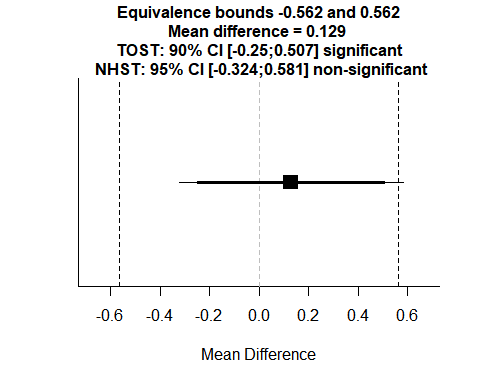
\includegraphics{manuscript_files/figure-latex/unnamed-chunk-8-1.pdf}
\caption{}
\end{figure}

\begin{verbatim}
## Using alpha = 0.05 Welch's t-test was non-significant, t(97.76702) = -1.07647, p = 0.2843664
## Using alpha = 0.05 the equivalence test based on Welch's t-test  was non-significant, t(97.76702) = 0.7054677, p = 0.2410984TOST results:
##   t-value 1 p-value 1 t-value 2   p-value 2       df
## 1 0.7054677 0.2410984 -2.858407 0.002601883 97.76702
## 
## Equivalence bounds (raw scores):
##   low bound raw high bound raw
## 1       -0.0625         0.0625
## 
## TOST confidence interval:
##   Lower Limit 90% CI raw Upper Limit 90% CI raw
## 1             -0.0960001              0.0204875
\end{verbatim}

We find that the TOST is non-significant, t(97.77) = 0.71, p = 0.24.
Thus, we cannot reject the possibility that the true effect really is
larger than our SESOI.\footnote{In this example, the bounds of the TOST
  was set based on a raw effect of 6.25\%. We could have converted this
  raw effect into a standardized effect (Cohen's d) for the current
  sample, and we would have gotten the exact same result, only then in
  Cohen's d (equivalence bounds = +/- 0.36). Since this is a replication
  of a previous study, we could also have chosen calculate the Cohen's d
  that corresponds to the raw SESOI in the \emph{original} study, and
  used this as the bounds for the replication. Now we would no longer be
  answering a question about a raw effect independent of the samples.
  Instead, we are asking whether we in the replication can reject
  standardized effects larger than a certain standardized effect in the
  original study. Since the standard deviations of the original study
  were only slightly higher than in the replication in this case,
  Cohen's d, and thus the bounds, would also be only sligthly smaller
  (bounds = +/- 0.34). As standard deviations of the original study
  compared to the replication becomes larger, the bounds become more
  narrow.}

\subsection{Example 4: Statistically Inferior and Not Statistically
Different}\label{example-4-statistically-inferior-and-not-statistically-different}

Lynott et al. (2014) conducted a study to investigate the effect of
being exposed to physically warm or cold stimuli on subsequent judgments
related to interpersonal warmth and prosocial behavior (replicating
Williams and Bargh, 2008). They observed that 51.2\% of participants who
received a cold pack (n = 427) opted to receive a reward for themselves,
while 57.9\% (n = 434) of participants who received a warm pack did the
same. Calculating a z-test for the difference between the proportions,
this effect is statistically significant (Diff = -0.067, z = -1.98, p =
0.024). Having obtained a significant result, we are left with two
alternatives:

\begin{enumerate}
\def\labelenumi{\arabic{enumi}.}
\tightlist
\item
  The difference is small enough that even though it is
  \emph{statistically} significant, we can consider it
  \emph{practically} equivalent to zero.
\item
  The difference is substantial enough that we cannot rule out that it
  is also practically significant.
\end{enumerate}

In this case, it is not really clear what an objective cirterion for the
smallest effect size of interest could be. However, since this is a
replication, we could decide that we do not care about an effect if the
difference is smaller than the smallest effect that the original study
could detect. This essentially means that we use the critical z value
(\textasciitilde{}1.96 in a two-tailed test with an alpha of 0.05) as
our bounds. To figure out what difference corresponds to a critical z in
the original study, we multiply critical z with the standard error:

\begin{verbatim}
## [1] 0.2510861
\end{verbatim}

Having determined the SESOI, we may also decide that since this is a
replication, we are only interested in whether the effect of receiving a
cold pack is significantly \emph{lower} than the smallest detectable
effect of the original study. In this case, we can still use a TOST to
analyse the data, but we only need to consider the test against the
upper bound because an effect with CIs crossing the lower bound can
still be \emph{lower} than the original effect.

\begin{figure}[htbp]
\centering
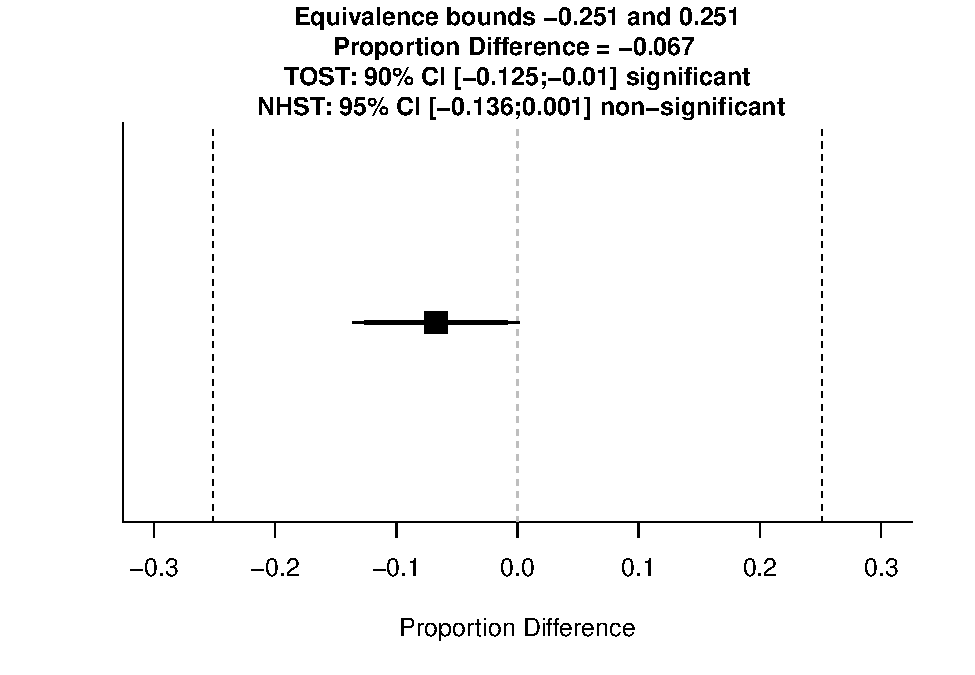
\includegraphics{manuscript_files/figure-latex/unnamed-chunk-10-1.pdf}
\caption{}
\end{figure}

\begin{verbatim}
## Using alpha = 0.05 Fishers exact z-test was non-significant, z = -1.925297, p = 0.05419224
## Using alpha = 0.05 the equivalence test based on Fishers exact z-test was significant, z = 5.274128, p = 6.669446e-08
## TOST results:
##   z-value 1    p-value 1 z-value 2    p-value 2
## 1  5.274128 6.669446e-08 -9.124721 3.596051e-20
## 
## Equivalence bounds:
##    low bound high bound
## 1 -0.2510861  0.2510861
## 
## TOST confidence interval:
##   Lower Limit 90% CI Upper Limit 90% CI
## 1         -0.1245121       -0.009780696
\end{verbatim}

We find that the test against the upper bound is significant, \(z =\)
-9.12, \(p =\) \textless{} 0.001. Thus, we can conclude that the
statistically non-significant effect is also statistically inferior to
our SESOI. \#\# Example 5: Not Statistically Equivalent and
Statistically Different Example 5: Correlations?

Would be nice to have 1 bounds based on effect sizes you have power to
detect. And one on just noticeable differences. This:
\url{http://wiki.ihe.net/images/e/e5/Measurement_of_pain.pdf} suggests
that this: Berry, H., Huskisson, E. C. Clin. Trials J. 1972, 9, 13. 12.
Hardy, J. D., Wolff, H. G., Goodell, H. Pain Sensations and Reactions.
Baltimore, 1952. shows that a VAS for pain can be divided into 20 just
noticeable differences' Or we use

\section{Adressing Trello cards}\label{adressing-trello-cards}

For the example where the results are inconclusive, explain how adding
more data, will, assuming the true effect is 0, lead to a smaller
confidence interval, and thus will lead to an informative test. However,
with increasing data, the effect could also slightly increase, to above
or at the SESOI level, and then the effect will be significant and not
equivalent. With massive amounts of data, many results will be
significant and equivalent.

\section{Discussion}\label{discussion}

The given examples and figures XXX to YYY illustrate that equivalence
testing is a relatively simple and flexible technique: As long as we can
calculate a confidence interval around a mean effect, we can compare it
to one or several bounds. In that sense, the result of an equivalence
test can be obtained by mere visual inspection of the CI (Seaman \&
Serlin, 1998; Tryon, 2001). This ease of use might tempt researchers to
set equivalence bounds after looking at their data. For example, we
showed above that Moon \& Roeder's replication of the identity-priming
study by Shih et al. (1999; example 3) does not exclude effects that are
large enough to affect a student's final grade on a test. However, if we
look at the \(90 \%\) CI (figure XXX), we can see that the data would
have been statistically equivalent if the bounds had been based on a
slightly larger SESOI, e.g.~a mean difference of 0.1. It is important to
point out that this strategy --- setting equivalence bounds \emph{based
on the obtained results} --- may be considered as \enquote{boundary
hacking}: Regardless of the underlying true effect, any finite CI will
exclude some values, which means that this procedure will lead to
capitalization on chance.

In order to avoid fooling ourselves more often than \(\alpha \%\) of the
time, equivalence bounds should be specified before results are known
(ideally as part of a preregistration; cf.~CONSORT guidelines, Piaggio
et al., 2006). A perhaps helpful guiding question may be: \enquote{Will
testing against these bounds yield interesting information in the long
run?} In most cases,

\section{Raw versus standardized equivalence
bounds}\label{raw-versus-standardized-equivalence-bounds}

Equivalence bounds can be set in terms of standardized effect sizes, or
raw differences. For example, the SESOI might be a raw mean difference
of 0.5 points on a 7-point scale, or a Cohen's d of 0.5. The main
difference is that equivalence bounds set in raw differences are
independent of the standard deviation, while equivalence bounds set as
standardized effects are dependent on the standard deviation (since they
are calculated as {[}FORMULA (X1-X2)/SD{]}. The observed standard
deviation randomly varies across samples. In practice, this means that
when you use standardized differences as bounds (e.g., d = 0.35) the
equivalence test depends on the standard deviation in the sample. The
equivalence bound for a raw mean difference of 0.5 equals a standardized
equivalence bound of d = 0.5 when the standard deviation is 1, but a
standardized equivalence bound of d = 1 then the standard deviation is
0.5.

Both raw equivalence bounds and standardized equivalence bounds have
specific benefits and limitations (for a discussion, see Baguley, 2009).
When raw mean differences are meaningful and of theoretical interest, it
makes sense to set equivalence bounds based on raw effect sizes. When
the raw mean difference is of less theoretical importance, or different
measures are used across research lines, it is often easier to set
equivalence bounds based on standardized differences. Researchers should
realize that equivalence bounds based on raw differences or standardized
differences ask slightly different questions, and justify their choice
for an equivalence bound. When setting equivalence bounds based on
earlier research, such as in replication studies, equivalence bounds
based on raw or standardized differences would ideally give the same
result, and large differences in standard deviations between studies are
as important to interpret as large differences in means.

\newpage

\section{References}\label{references}

Button, K. S., Kounali, D., Thomas, L., Wiles, N. J., Peters, T. J.,
Welton, N. J., . Lewis, G. (2015). Minimal clinically important
difference on the Beck Depression Inventory - II according to the
patient's perspective. Psychological Medicine, 45(15), 3269-3279.
\url{https://doi.org/10.1017/S0033291715001270}

Burriss, R. P., Troscianko, J., Lovell, P. G., Fulford, A. J. C.,
Stevens, M., Quigley, R., . Rowland, H. M. (2015). Changes in Women's
Facial Skin Color over the Ovulatory Cycle are Not Detectable by the
Human Visual System. PLOS ONE, 10(7), e0130093.
\url{https://doi.org/10.1371/journal.pone.0130093}

Lakens, D. (2017). Equivalence Tests: A Practical Primer for t Tests,
Correlations, and Meta-Analyses. Social Psychological and Personality
Science, 8(4), 355--362.

\hypertarget{refs}{}
\hypertarget{ref-lakens_equivalence_2017}{}
Lakens, D. (2017). Equivalence Tests: A Practical Primer for t Tests,
Correlations, and Meta-Analyses. \emph{Social Psychological and
Personality Science}, \emph{8}(4), 355--362.
doi:\href{https://doi.org/10.1177/1948550617697177}{10.1177/1948550617697177}






\end{document}
